\documentclass{article}
\usepackage[utf8]{inputenc}
\usepackage{enumitem}
\usepackage{xcolor}
\usepackage{geometry}
\usepackage{titling}
\usepackage{sectsty}
\usepackage{graphicx}
\usepackage{natbib}
\usepackage{hyperref} 


\geometry{a4paper, margin=1in}
\definecolor{darkblue}{rgb}{0.0, 0.0, 0.55}

\title{\color{darkblue}\LARGE Service Workers}
\author{Jesus Armando Gomez Leyva}

\pretitle{\begin{center}\LARGE\bfseries}
\posttitle{\par\end{center}\vskip 0.5em}

\begin{document}

\maketitle

\section*{\color{darkblue}\Large Introduction}

The Service Worker API is a powerful tool that empowers web developers to create highly functional and responsive web applications. Essentially acting as intermediary servers, service workers sit between the web application, the browser, and the network infrastructure, facilitating a range of advanced functionalities like  to enable the creation of effective offline experiences, intercept network requests and take appropriate action based on whether the network is available, and update assets residing on the server.
\citep{ServiceWorker}


\begin{figure}[h]
    \centering
    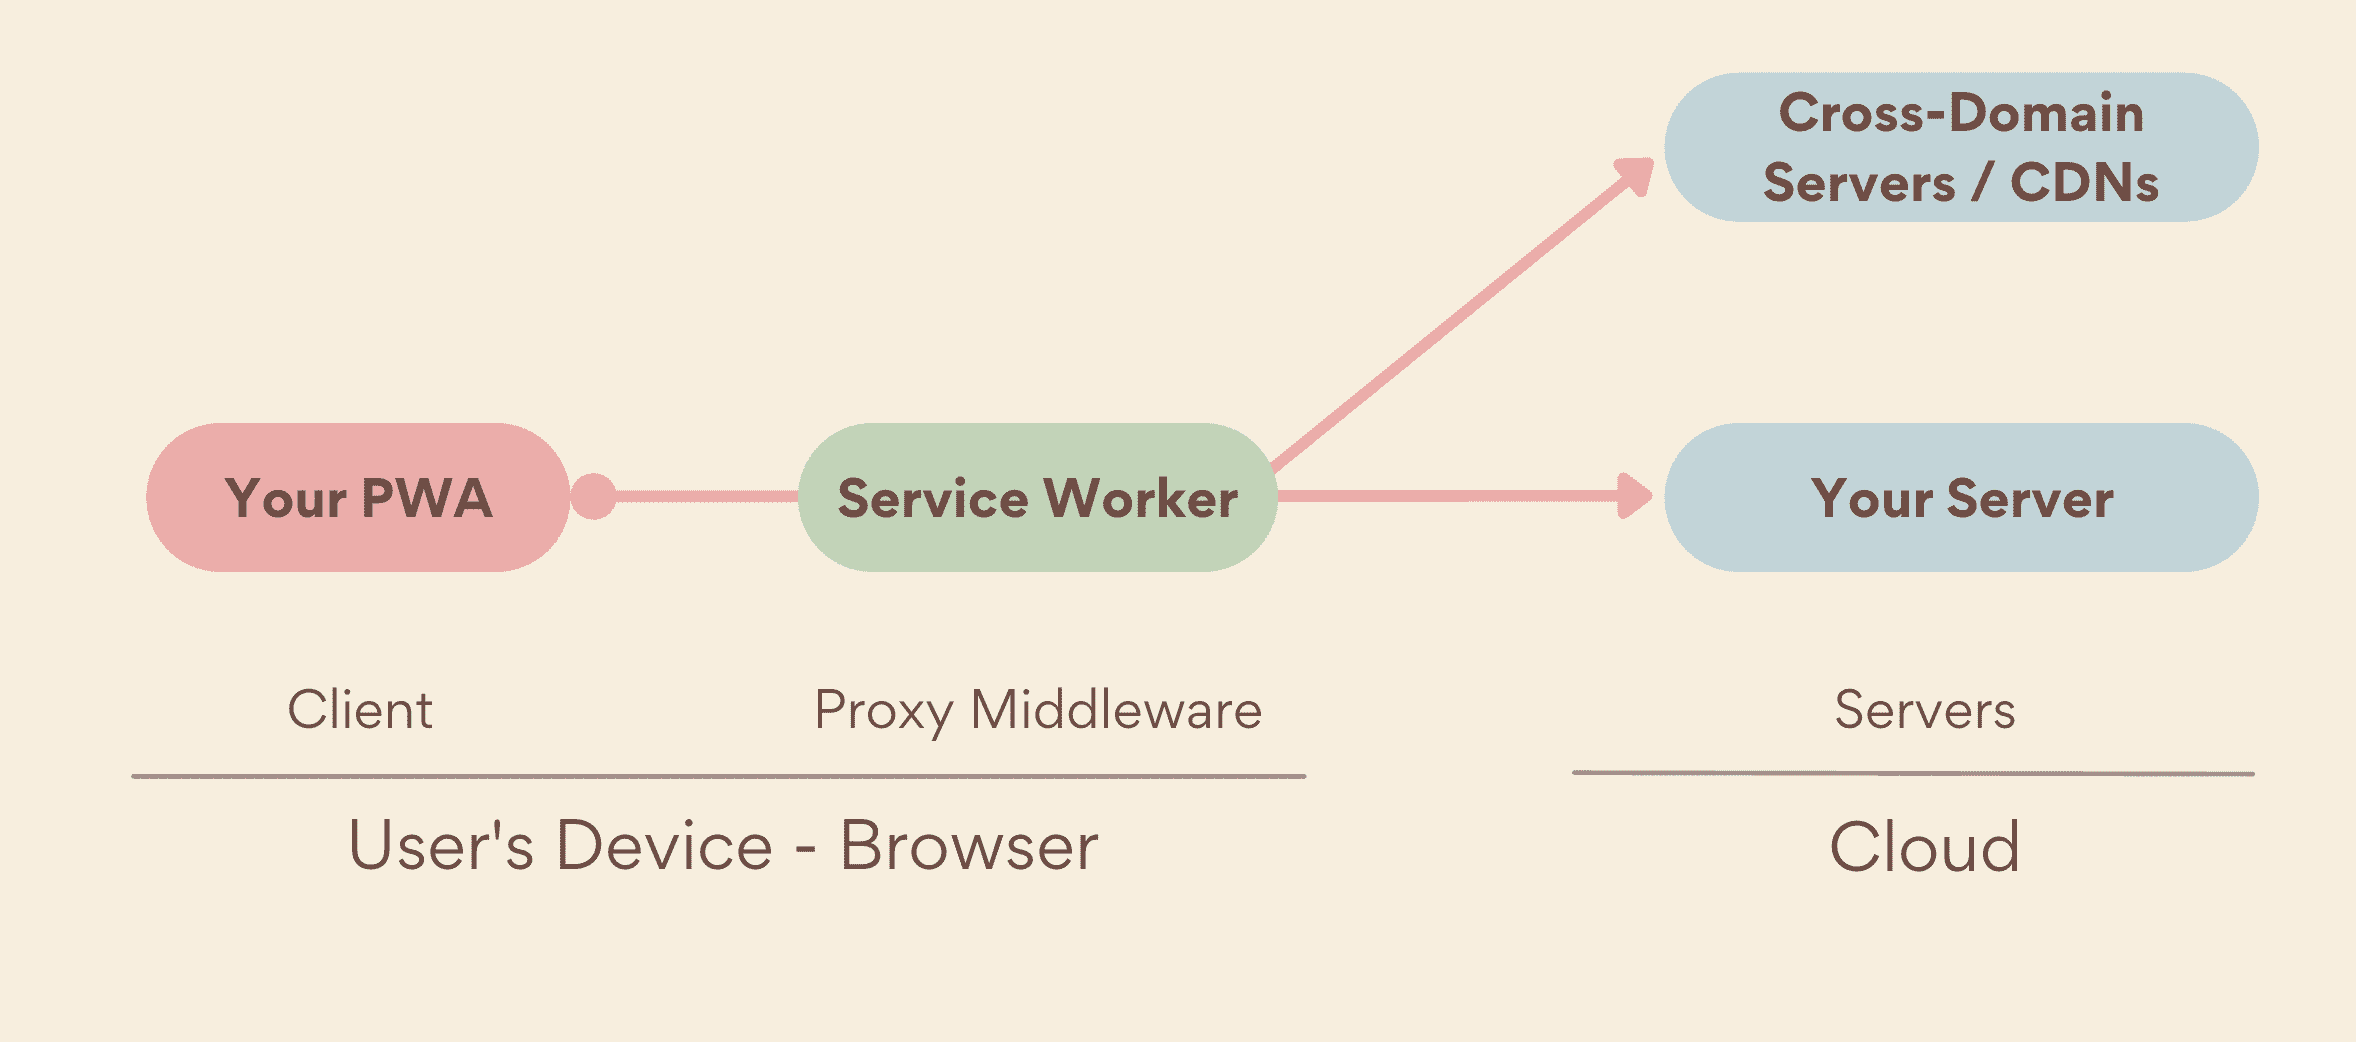
\includegraphics[width=1\textwidth]{images/serviceworker.png}

\end{figure}

\section*{\color{darkblue}\Large Goals and Characteristics}

\begin{itemize}[label=$\bullet$, leftmargin=*]
    \item \textbf{Offline Experiences:} Service workers enable effective offline experiences by intercepting network requests and taking appropriate actions based on network availability.
    \item \textbf{Event-Driven Workers:} They operate as event-driven workers registered against specific origins and paths within web applications.
    \item \textbf{Separation of Concerns:} Service workers function independently from the main thread of the application, enhancing security and separation of concerns.
    \item \textbf{Limited DOM Access:} They lack direct access to the Document Object Model (DOM) and communicate with the main application thread using message passing.
\end{itemize}

\section*{\color{darkblue}\Large Use Cases}

\begin{itemize}[label=$\bullet$, leftmargin=*]
    \item \textbf{Offline Functionality:} Craft seamless user experiences even in offline or poor network conditions.
    \item \textbf{Background Data Synchronization:} Enable background data synchronization for enhanced user experience.
    \item \textbf{Resource Requests:} Respond to resource requests from other origins.
    \item \textbf{Performance Optimization:} Pre-fetch resources and optimize performance by efficiently fetching resources from the server.
\end{itemize}

\citep{Medium}
\section*{\color{darkblue}\Large Conclusion}

Service workers are a versatile and powerful tool for web developers, providing granular control over web application behavior in various network conditions. They enable the creation of sophisticated offline experiences and performance optimizations, ultimately enhancing the user experience.

\bibliographystyle{plainnat}
\bibliography{references}



\end{document}
